\documentclass{sig-alternate}
\usepackage{color}
\usepackage[colorinlistoftodos]{todonotes}
\usepackage{algorithm}
\usepackage[noend]{algpseudocode}

\newtheorem{theorem}{Theorem}




%%%%% Uncomment the following line and comment out the previous one
%%%%% to remove all comments
%%%%% NOTE: comments still occupy a line even if invisible;
%%%%% Don't write them as a separate paragraph
%\newcommand{\mycomment}[1]{}

\begin{document}

\conferenceinfo{UMM CSci Senior Seminar Conference, April 2017}{Morris, MN}

\title{Conflict-Free Vertex Coloring Of Planar Graphs}

\numberofauthors{1}

\author{
\alignauthor
Shawn S. Seymour\\
	\affaddr{Division of Science and Mathematics}\\
	\affaddr{University of Minnesota, Morris}\\
	\affaddr{Morris, Minnesota, USA 56267}\\
	\email{seymo079@morris.umn.edu}
}

\maketitle
\begin{abstract}
The conflict-free coloring problem is a variation of the vertex coloring problem, a classical NP-hard optimization problem. The conflict-free coloring problem aims to color the vertices of a graph in a way where every vertex is connected to at least one uniquely colored vertex. This paper presents heuristics to solve the conflict-free coloring problem on both general graphs and planar graphs. This paper also looks into bounds on the number of colors needed.
\end{abstract}

\section{Introduction}
\label{sec:introduction}

Consider the map of the 48 contiguous states in the United States of America. Suppose we would like to color each state such that no two states that share a boundary have the same color. This problem can be modeled with a graph. We can represent each state with a \emph{vertex} and represent a boundary between two states with an \emph{edge}. This map is an example of a planar graph, i.e. none of the edges cross when drawn on a plane.

This is a famous example of the \emph{vertex coloring} problem and one of many graph coloring problems. The vertex coloring problem aims to find the minimum number of colors needed to color a graph such that no two adjacent vertices are colored with the same color. While some problems are relatively easy to solve, the vertex coloring problem is one of the most computationally complex problems in computer science and mathematics. The vertex coloring problem has many real-world applications such as exam timetabling, register allocation, and the scheduling of taxis.

The \emph{conflict-free coloring} problem is a relaxed variation of the vertex coloring problem. The conflict-free coloring problem does not aim to color every vertex such that it is not connected to a vertex of the same color. Rather, it aims to color \emph{enough} vertices such that for every vertex, it is connected to at least one uniquely colored vertex.

This paper looks into some applications and heuristics of conflict-free coloring. We then look into the specific case of conflict-free coloring planar graphs. Section 2 provides background necessary to understand the problem and how it is used. Section 3 introduces some applications for the conflict-free coloring problem. Section 4 describes a heuristic for conflict-free coloring general graphs. Section 5 looks into the specific case of conflict-free coloring planar graphs.


\section{Background}
\label{sec:background}
To understand the problem, the algorithms to solve it, and its results, we must first understand some graph theory, some computational complexity theory, and the precise definitions of the vertex coloring problem and the conflict-free coloring problem.

\begin{figure}[h]
	\centering
	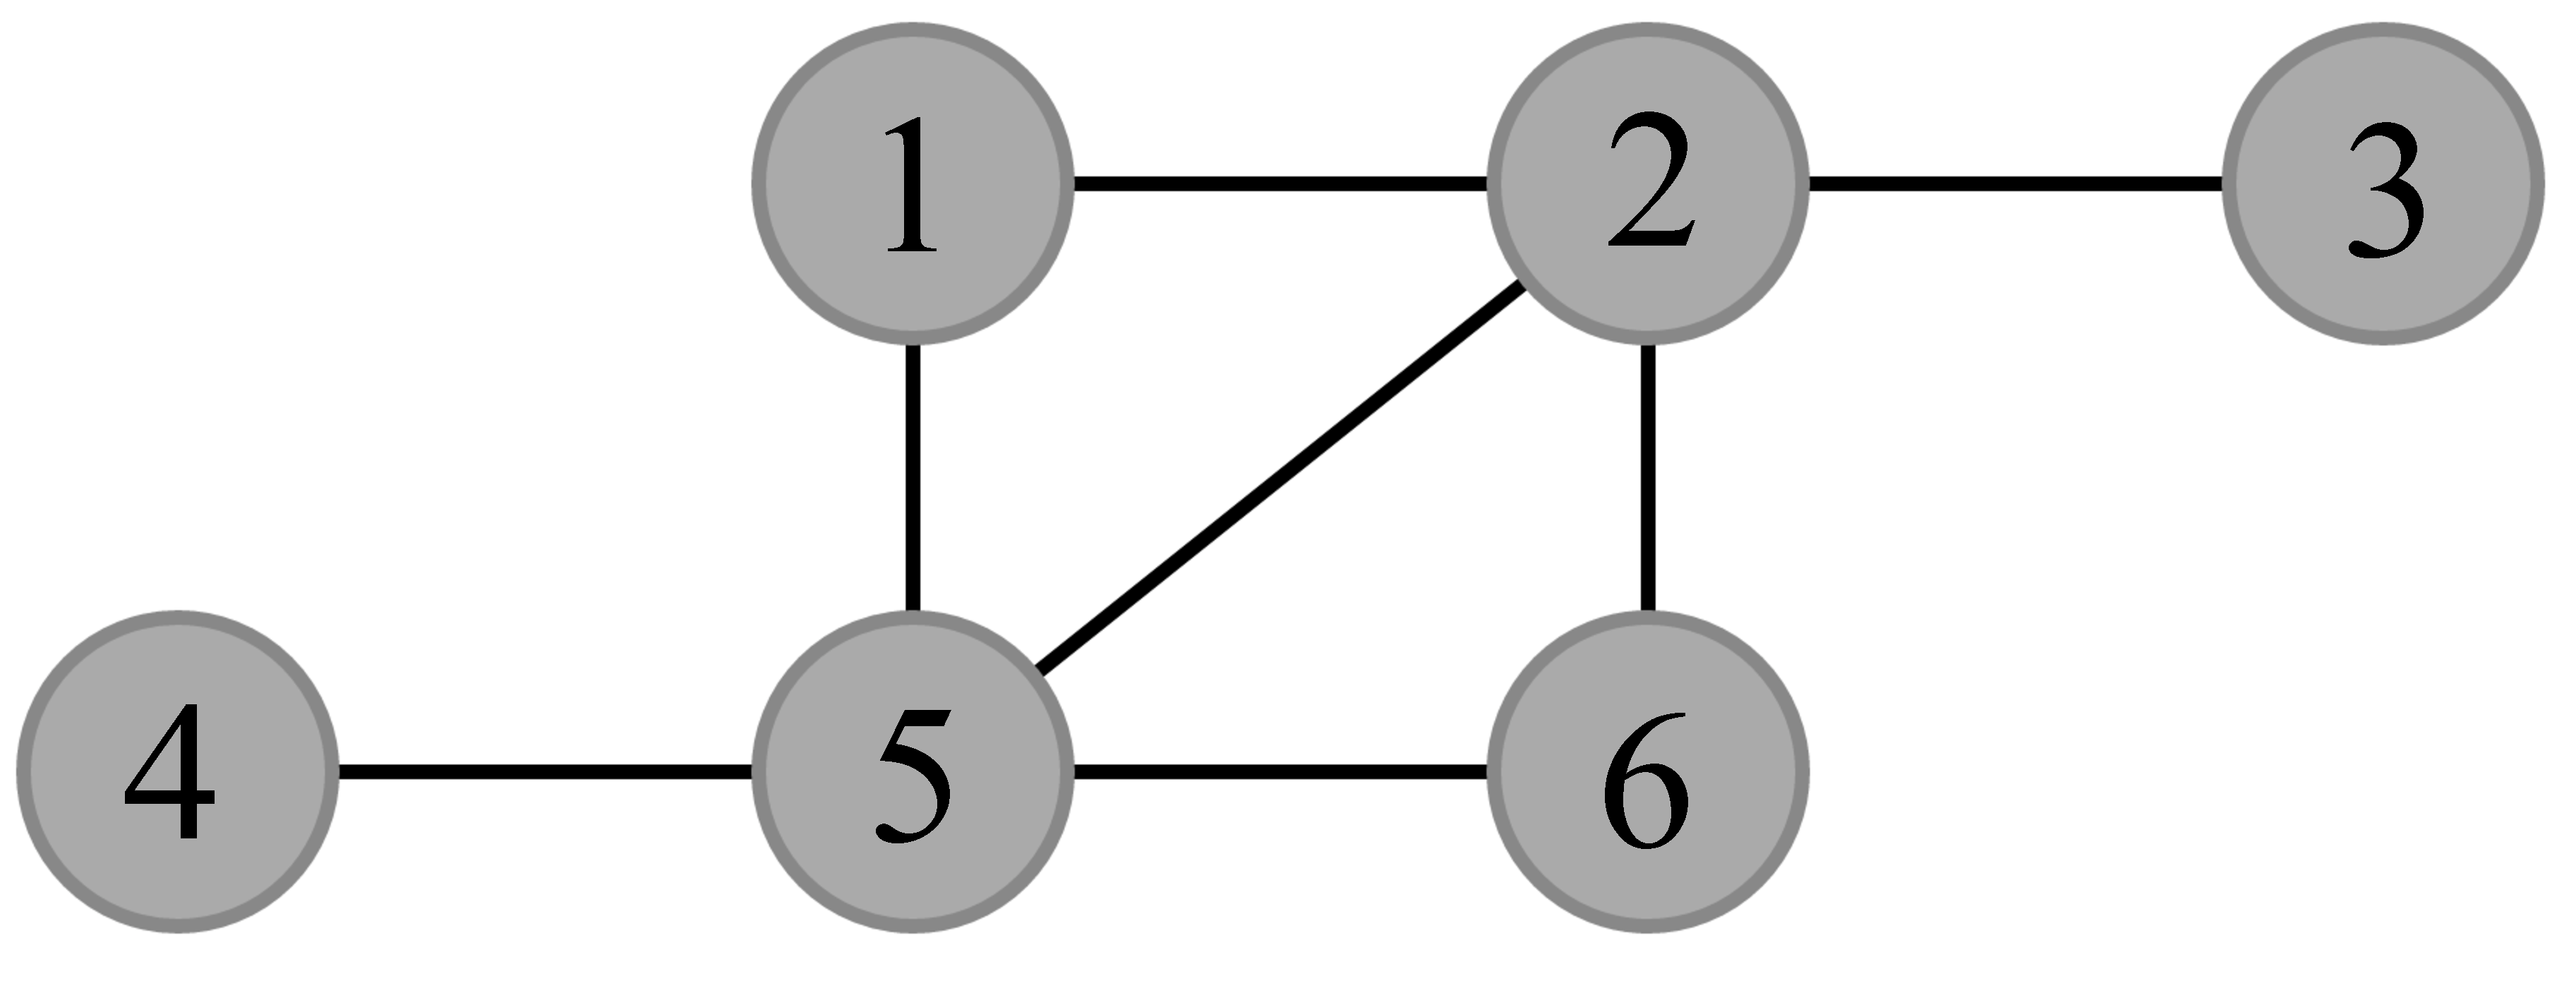
\includegraphics[width=7cm]{../figures/example.pdf}
	\caption{A simple, undirected graph $G_1$}\label{fig:graph}
\end{figure}

\subsection{Graph Theory}
\label{sec:graphtheory}

A graph, denoted $G=(V,E)$, is an ordered pair of two sets: a set of vertices $V$ and a set of edges $E$. Each edge consists of a pair of vertices from $V$. For example, $(u,w) \in E$ is an edge connecting vertices $u$ and $w$ where $u,w \in V$. Vertices are adjacent if they are connected by an edge. A simple graph is an undirected graph where each edge connects two different vertices and no two edges connect the same pair of vertices. All graphs used by the vertex coloring problem and conflict-free coloring problem will be undirected, simple graphs. An example graph that we will use later on is shown in figure \ref{fig:graph}.

The neighborhood of a vertex, denoted $N_G(v)$, is a set of all vertices adjacent to $v$. A \emph{closed} neighborhood consists of all vertices adjacent to $v$ and $v$ itself. Unless stated otherwise, we will assume when talking about neighborhoods that they are closed neighborhoods. The degree of a vertex, denoted $d_G(v)$, is the number of vertices adjacent to $v$. The maximum degree of a graph $G$, denoted $\Delta(G)$, is the maximum degree of its vertices. \cite{bondy1976graph}

\begin{figure}[h]
	\centering
	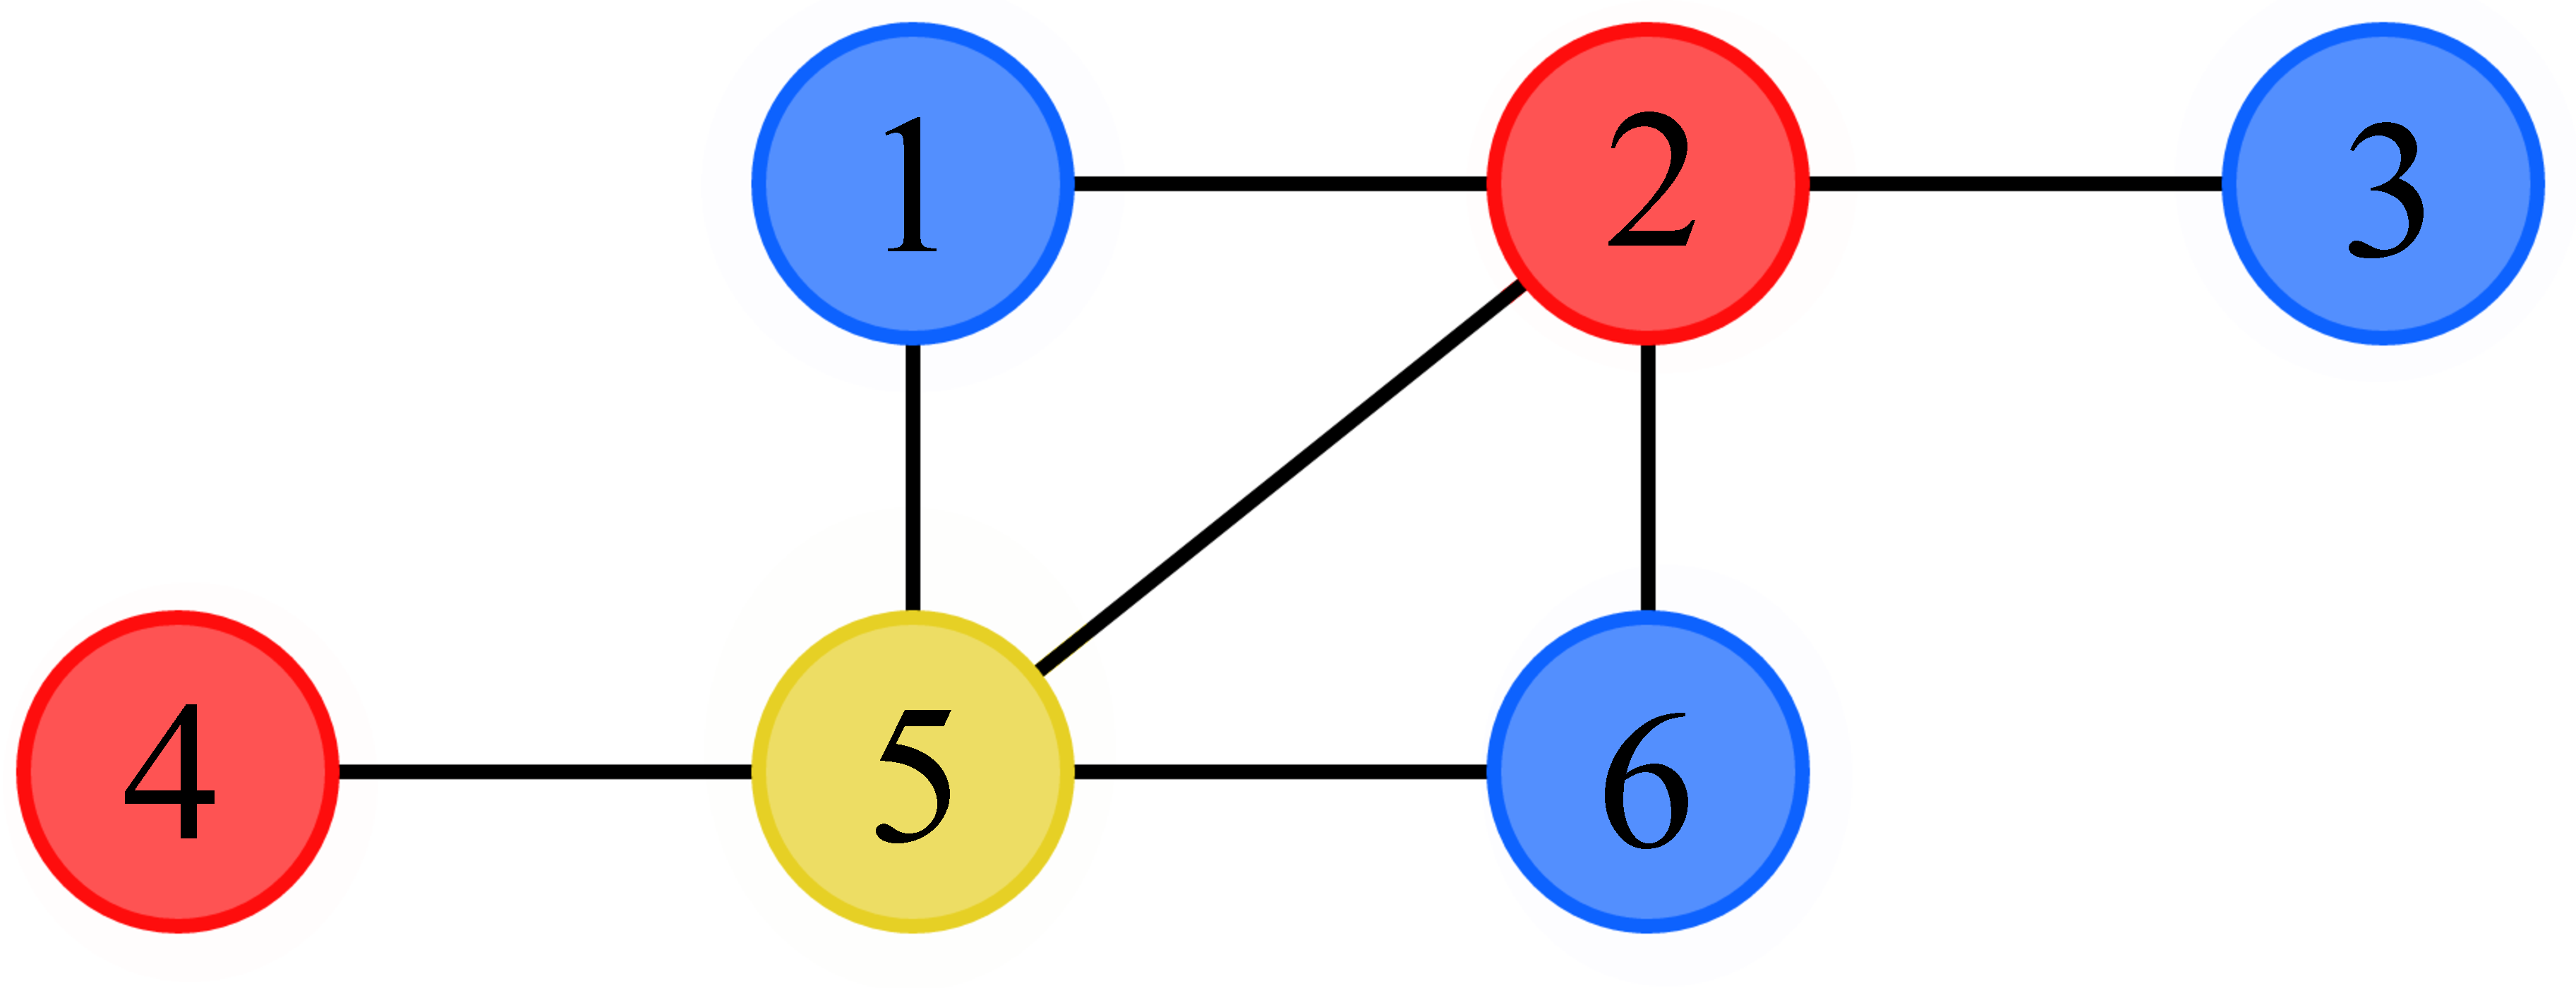
\includegraphics[width=7cm]{../figures/example-vcp.pdf}
	\caption{A minimum vertex coloring of $G_1$}\label{fig:vcp-example}
\end{figure}

\todo[inline]{The figures will be shaded with angled lines eventually}

\subsection{Graph Coloring}
\label{sec:coloring}
A vertex coloring is an assignment of colors to each vertex of a graph $G$ such that no adjacent vertices share the same color. Mathematically, it can be described as a function $f : V \rightarrow S = \{1, 2, \dots, k\}$ such that $\forall u,w \in V$, if $(u,w) \in E$, then $f(u) \neq f(w)$. A vertex coloring that satisfies this constraint is called a \emph{proper coloring}. The \emph{chromatic number} of $G$, denoted $\chi(G)$, is the minimum number of colors, i.e. $|S|$, needed to properly color $G$. The \emph{vertex coloring} problem, when given a simple graph $G$, is to find $\chi(G)$. \cite{bondy1976graph}

A graph $G$ is said to be \emph{k-colorable} if it can be colored using $k$ or fewer colors, i.e. $\chi(G) \leq k$. A graph having $\chi(G) = k$ is said to be a \emph{k-chromatic} graph. The \emph{k-colorability} problem asks if a graph can be colored using $k$ colors. This problem is a slightly easier problem than the vertex coloring problem as it is decision problem rather than an optimization problem. An example of a 3-colorable graph and a vertex coloring is shown in figure \ref{fig:vcp-example}.

\begin{figure}[h]
	\centering
	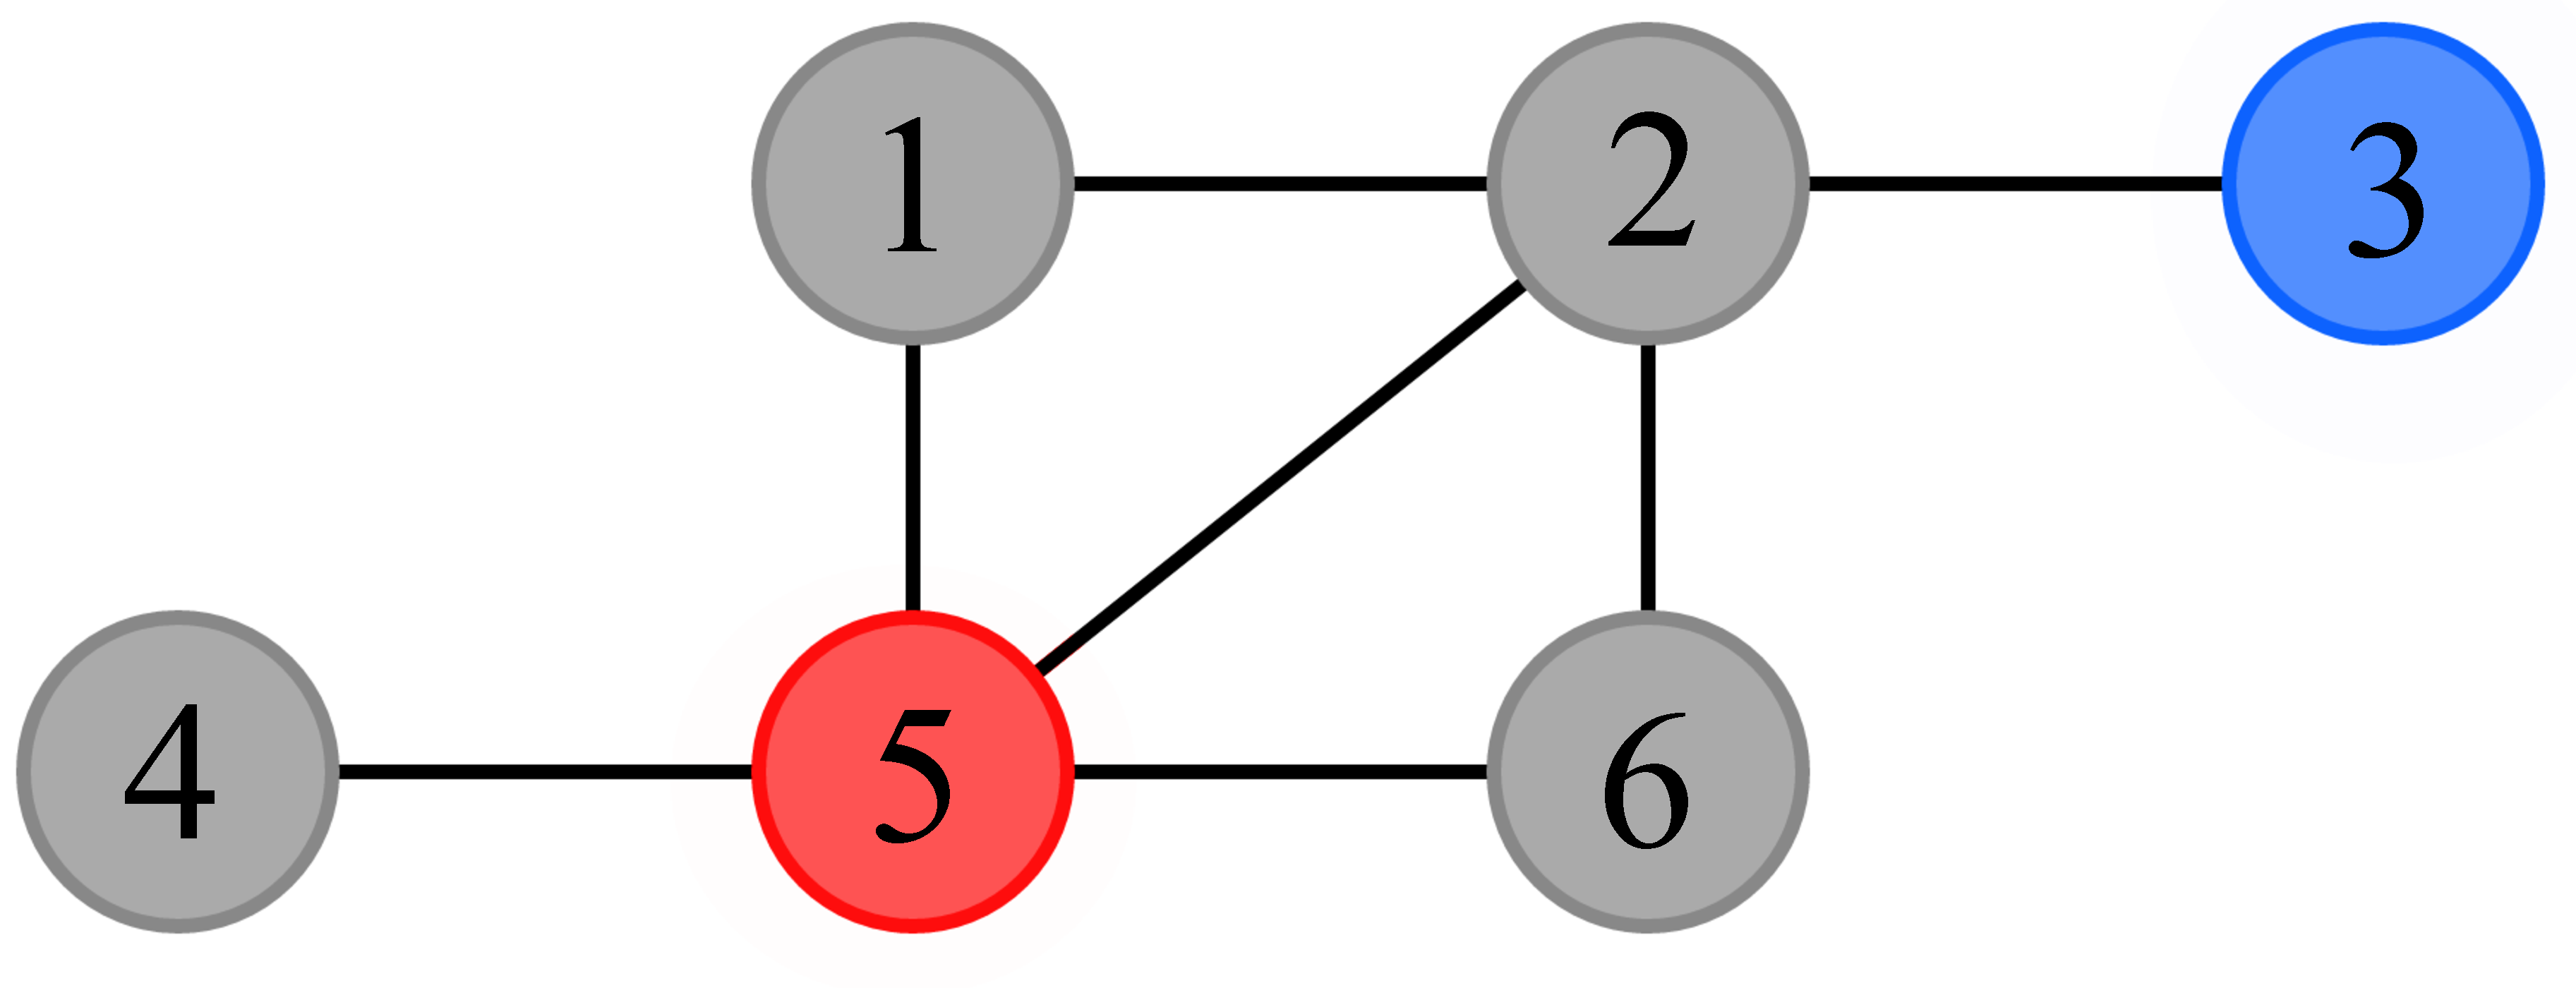
\includegraphics[width=7cm]{../figures/example-cfcp.pdf}
	\caption{A minimum conflict-free coloring of $G_1$}\label{fig:cfcp-example}
\end{figure}

A \emph{conflict-free coloring} of a graph assigns one of $k$ colors to some of the vertices such that, for every vertex $v$, there is a unique color assigned to a vertex among $v$ and $v$'s neighbors. A \emph{conflict-free k-coloring} of a simple graph $G$ assigns one of $k$ different colors to a subset $S \subseteq V$ of vertices such that $\forall v \in V$, there is a vertex $u \in N(v)$ where the color of $u$ is unique in the closed neighborhood of $v$. The vertex $u$ can be thought of the \emph{conflict-free neighbor} of $v$. The \emph{conflict-free chromatic number} of G, denoted $\chi_{CF}(G)$, is the smallest $k$ for which a conflict-free coloring exists. \cite{abel2017three}

An example of a conflict-free coloring is shown in figure \ref{fig:cfcp-example}. It is worth noting that all proper vertex colorings are also conflict-free colorings. This is because in a proper vertex coloring, every vertex is its own conflict-free neighbor \cite{abel2017three}. We observe from figures \ref{fig:vcp-example} and \ref{fig:cfcp-example}, $\chi(G_1) = 3$ and $\chi_{CF}(G_1) = 2$.

The domination number of $G$, denoted $\gamma(G)$, is the size of a minimum dominating set of G. A dominating set is a subset $D$ of $V$ such that every vertex not in $D$ is adjacent to at least one vertex in $D$. The \emph{conflict-free domination number} for some $k$, denoted $\gamma_{CF}^k(G)$, is the minimum number of vertices that have to be colored in a conflict-free k-coloring of $G$. An example of a dominating set is $\{3, 5\}$ of graph $G_1$ where $\gamma(G_1) = 2$.

\subsection{Computational Complexity Theory}
\label{sec:complexitytheory}
A \emph{decision} problem, as mentioned earlier, is a problem that can be answered with a `yes' or a `no' \cite{sipser2006introduction}. A decision problem is said to be in the class \emph{P} if in the worst case, it can be solved with an algorithm that runs in polynomial time. A problem can be solved in polynomial time if an algorithm with input size $n$ can run in at most $n^k$ steps where $k$ is a constant that does not depend on $n$.

Given a decision problem and information showing what the answer is, it can be possible to verify the answer quickly. If a decision problem can be verified in polynomial time but not necessarily solved in polynomial time, it is said to be in the class \emph{NP}. Take note that this does not exclude problems in class \emph{P}; \emph{P} is a subset of \emph{NP}.

There are certain problems that can be proven to be as hard as every problem in NP. There problems are said to be NP-hard. A problem is NP-hard if it every problem in NP can be polynomially reduced to it. This brings an important result: if an NP-hard problem can be solved with an algorithm that runs in polynomial time, then any problem in NP could be solved in polynomial time. A decision problem is said to be \emph{NP-complete} when it is both in NP and NP-hard.

The vertex coloring problem (VCP) and the conflict-free coloring problem (CFCP) are not in the class NP as they are not decision problems. A common approach to proving problems as NP-hard or NP-complete is a reduction from a known NP problem. If we find a known hard problem $Y$, then we can prove that another problem $X$ is hard by reducing $Y$ to $X$. The VCP and the CFCP have both been shown to be NP-hard \cite{abel2017three,moret1998theory}. The \emph{k-colorability} problem is proven to be NP-complete with a reduction from 3-SAT, a well-known NP-complete problem \cite{sharma2012new}.

\section{Applications}
Before digging into methods for solving the conflict-free coloring problem, it is important to understand why conflict-free coloring is useful. It is useful to know what motivated the recent studies into conflict-free coloring.

\subsection{Wireless Networks}
The main application for conflict-free coloring surrounds wireless networks. Cellular networks, radio, television broadcasting, and satellite communication utilize some form of wireless networks. For each of these systems, a frequency assignment problem arises with specific characteristics.

For example, imagine a cellular network. Cellular networks are heterogeneous networks with two different types of nodes. They have \emph{base-stations} (servers) and \emph{clients}. Base stations are all interconnected through an external backbone network. Clients can only be connected to base stations and connect via radio links. Base stations are each assigned a fixed frequency. Clients, however, are constantly searching frequencies in search for base-stations with good reception.

The problem when initially setting up these networks comes into play when assigning frequencies. Imagine two base-stations near each other having the same frequency. If a client is in reception range of both base-stations, then mutual interference occurs and the radio link is too noisy to be used for proper communication. The goal is to assign frequencies to base stations such that every client is served by some base-station and to minimize the number of frequencies used.

This problem was initially modeled as a vertex coloring problem, where the vertices are the base-stations and the edges are the pairs of base-stations that overlap in their reception range. This model is too wasteful and restrictive. Imagine a situation where a client is within the reception range of 3 base-stations. The VCP model would require 3 colors, one for each base station. If we assign one base-station a color (say blue) and the other 2 (say red), then we only utilize two colors and the client utilizes the blue base-station and has no mutual interference. This model is shown in figure \ref{fig:towers}. This is exactly what a conflict-free coloring does. \cite{smorodinsky2013conflict}

\begin{figure}[h]
	\centering
	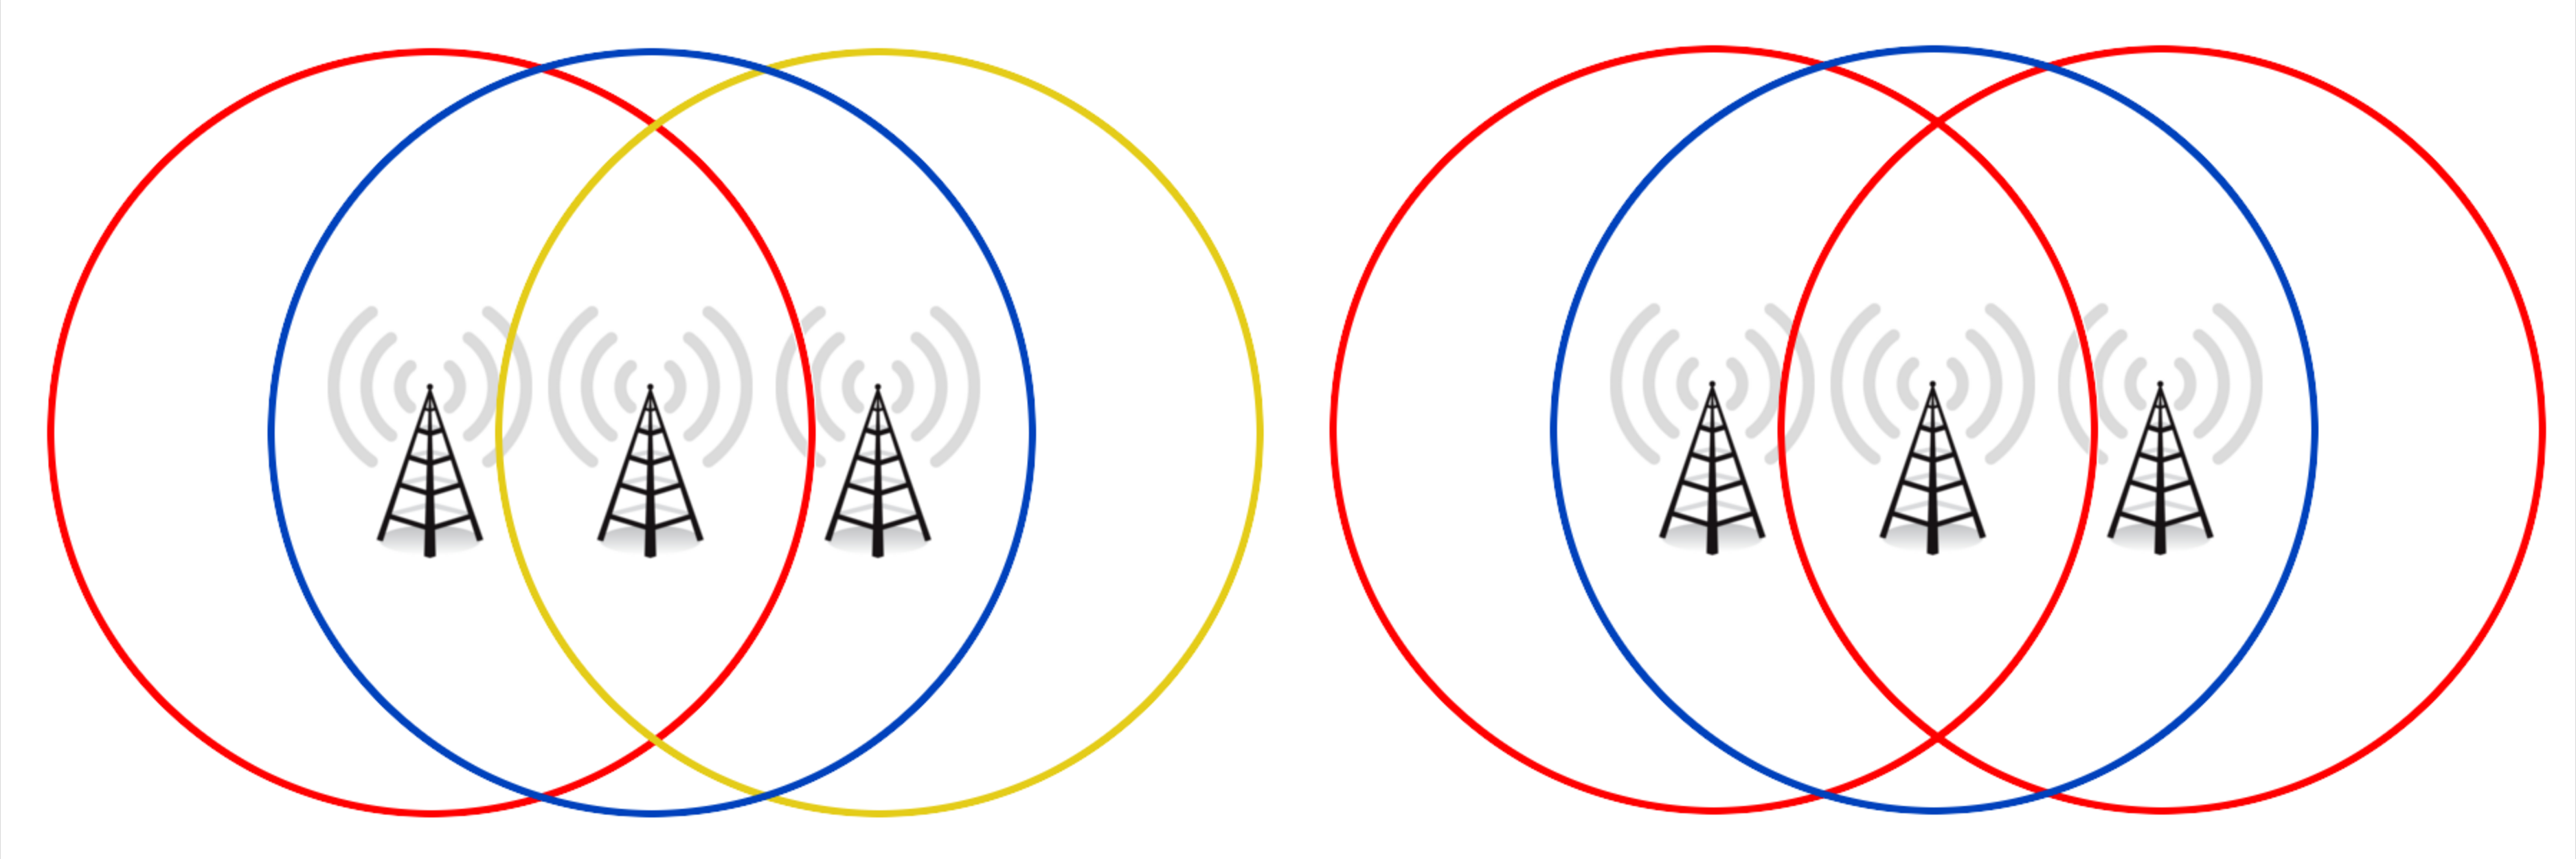
\includegraphics[width=8cm,trim=4 4 4 4,clip]{../figures/towers.pdf}
	\caption{Cellular tower VCP and CFCP example}\label{fig:towers}
\end{figure}

\subsection{RFID Networks}
Radio frequency identification (RFID) networks are similar to wireless networks. An object, such as a credit card with an RFID chip, has a specific tag attached to it. A reader, such as a credit card scanner, can sense the presence of this object and read an ID that is assigned to the tag of the object. RFID is used for tracking progress of automobiles through a production assembly line, timing marathons and races, security access control to parking garages and buildings, and much more.

Multiple RFID readers are often setup in a given location to improve coverage of the overall area. There can also be multiple RFID readers set up that each do a different action after reading a tagged object. Unlike cellular towers, a reader can only be reading (i.e. connected to) a single tag at a time. Two readers trying to access a tagged object at the same time can cause mutual interference. The goal is to schedule for each reader a time slot for when the reader will be active.

Imagine we have a set of readers, $R$. Suppose they all are assigned the same frequency. We would like to schedule each reader $r \in R$ a time slot $t(r)$ where the reader $r$ will be active. We have a set of tags $P$ (i.e. automobile RFID chips). We can say that $P$ is read by our schedule if for every tag $p \in P$, there is at least one reader $r \in R$ and a time $t$ such that $p$ is read by $r$ at time $t$. We want to minimize the total time slots used by the schedule. This can be accomplished by modeling the situation as a conflict-free coloring problem. Again, we aim to find the minimum number of colors needed.

\section{CF Coloring of General Graphs}
For the rest of this paper, we will consider the NP-complete problem of conflict-free k-colorability. Given a graph $G$ and an integer $k$, determine if graph $G$ can be colored using $k$ or fewer colors. Although all graphs can be conflict-free colored, a given graph $G$ may not be able to be colored with $k$ colors.

As shown with graph $G_1$ in section \ref{sec:background}, even though all proper vertex colorings are also conflict-free colorings, fewer colors can usually be used. This leads us to use heuristics that differ from the vertex coloring problem. Abel et al. \cite{abel2017three} present an efficient heuristic to color certain general graphs with $k$ colors in a conflict-free manner. They call this heuristic \emph{iterated elimination of distance-3-sets}.

\subsection{Guaranteeing CF k-Colorability}
It is wasteful to spend time coloring a graph that cannot be conflict-free colored. This leads Abel et al. to provide sufficient criterion to guarantee the conflict-free k-colorability of a certain graphs. To introduce this criterion, we need to introduce a few specific graphs. A complete graph is a simple, undirected graph where every pair of distinct vertices is connected by an edge. A complete graph on $n$ vertices is denoted as $K_n$. The graph $K_n^{-3}$ is the graph obtained by removing any three edges forming a single triangle, i.e. \(K_n^{-3} =  \left ( V(K_n), E(K_n) \setminus E(K_3) \right ) \). A graph $H$ is called a \emph{minor} of a graph $G$ if $H$ can be formed from $G$ by deleting edges and vertices and by contracting edges. \cite{abel2017three,bondy1976graph}

\begin{theorem} \label{thm:criterion}
Let $G$ be a graph and $k \geq 1$. If $G$ has neither $K_{k+2}$ nor $K_{k+3}^{-3}$ as a minor, $G$ has a conflict-free coloring that can be found in polynomial time using iterated elimination of distance-3-sets.
\end{theorem}

Abel et al. give a criterion that guarantees k-colorability which is stated in theorem \ref{thm:criterion}. In the proof of this theorem, found in \cite{abel2017three}, the authors prove that their heuristic will always generate a k-colorable graph when the specified criterion is met. To illustrate this heuristic, we will generate a graph that fits the specified criterion and apply the iterated elimination of distance-3-sets algorithm defined as algorithm \ref{alg:elimination}.

\subsection{Setting Up Example CF Coloring}
We will demonstrate meeting the criterion to utilize this algorithm using the graph $G_2$ in figure \ref{fig:criterion}.

\begin{figure}[h]
	\centering
	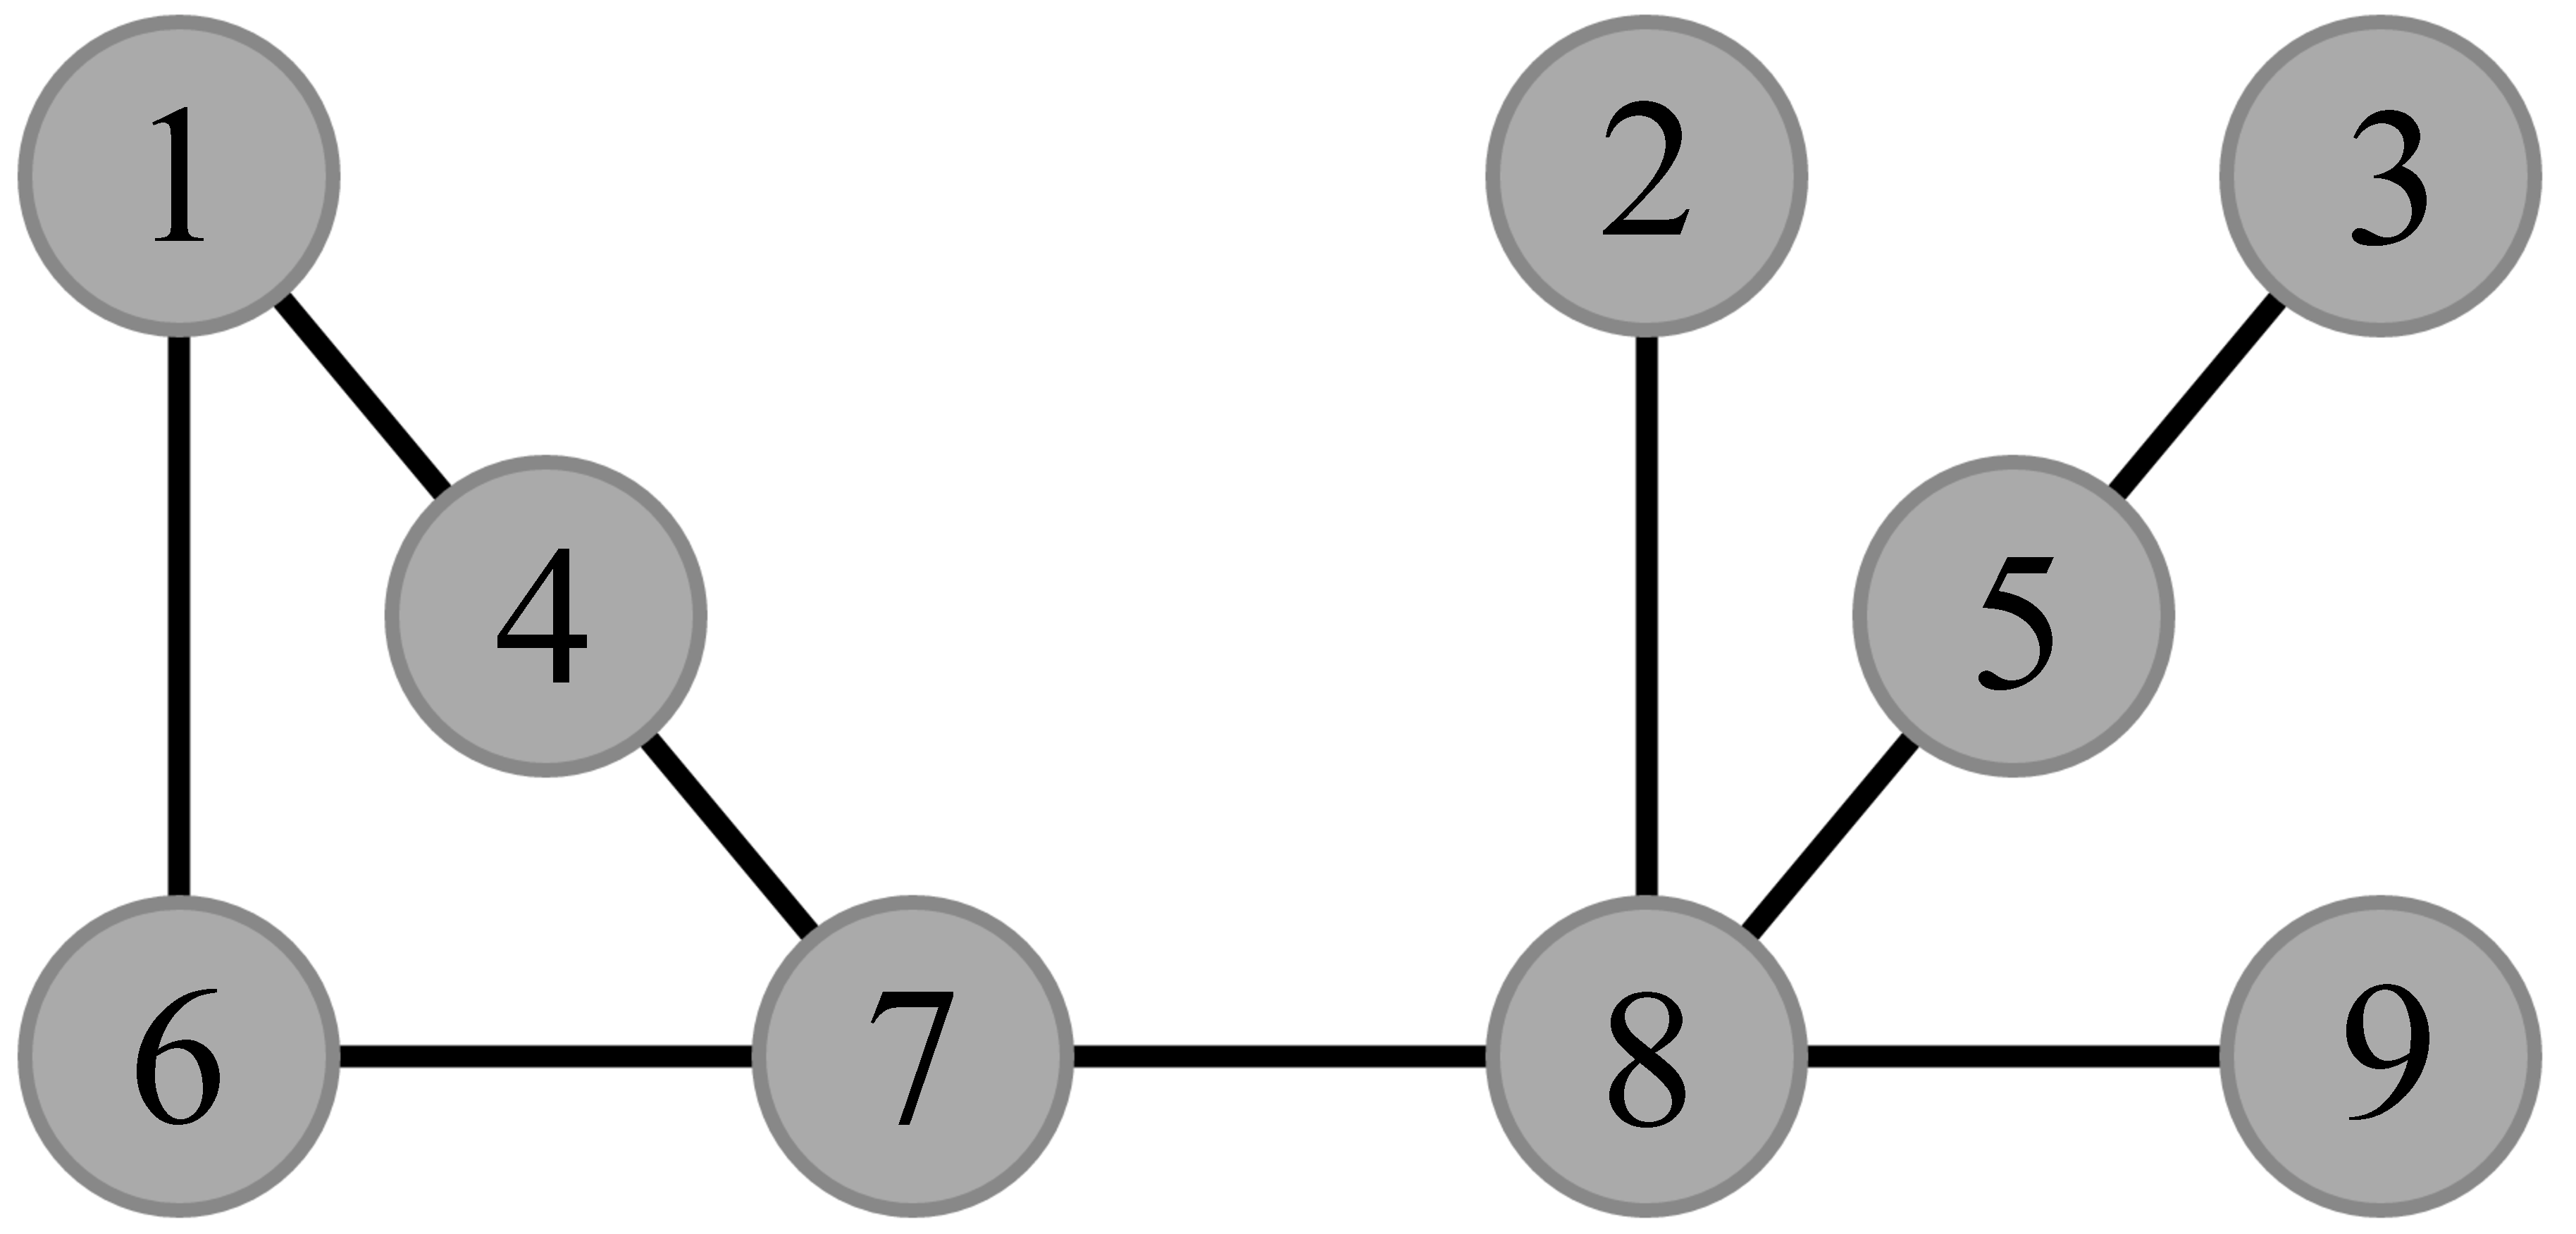
\includegraphics[width=6cm]{../figures/criterion.pdf}
	\caption{A simple graph $G_2$}\label{fig:criterion}
\end{figure}

We will be focusing on the simplest example, $k = 1$. Graph $G_2$ is a simple graph with 6 vertices. It does not, however, fit our criterion; it actually breaks both properties as it has both $K_{k+2}$ and $K_{k+4}^{-3}$ as a minor. For $k = 1$, this means our graph cannot contain $K_{3}$ or $K_{4}^{-3}$ as a minor. These graphs are shown in figure \ref{fig:bad-criterion}.

\begin{figure}[h]
	\centering
	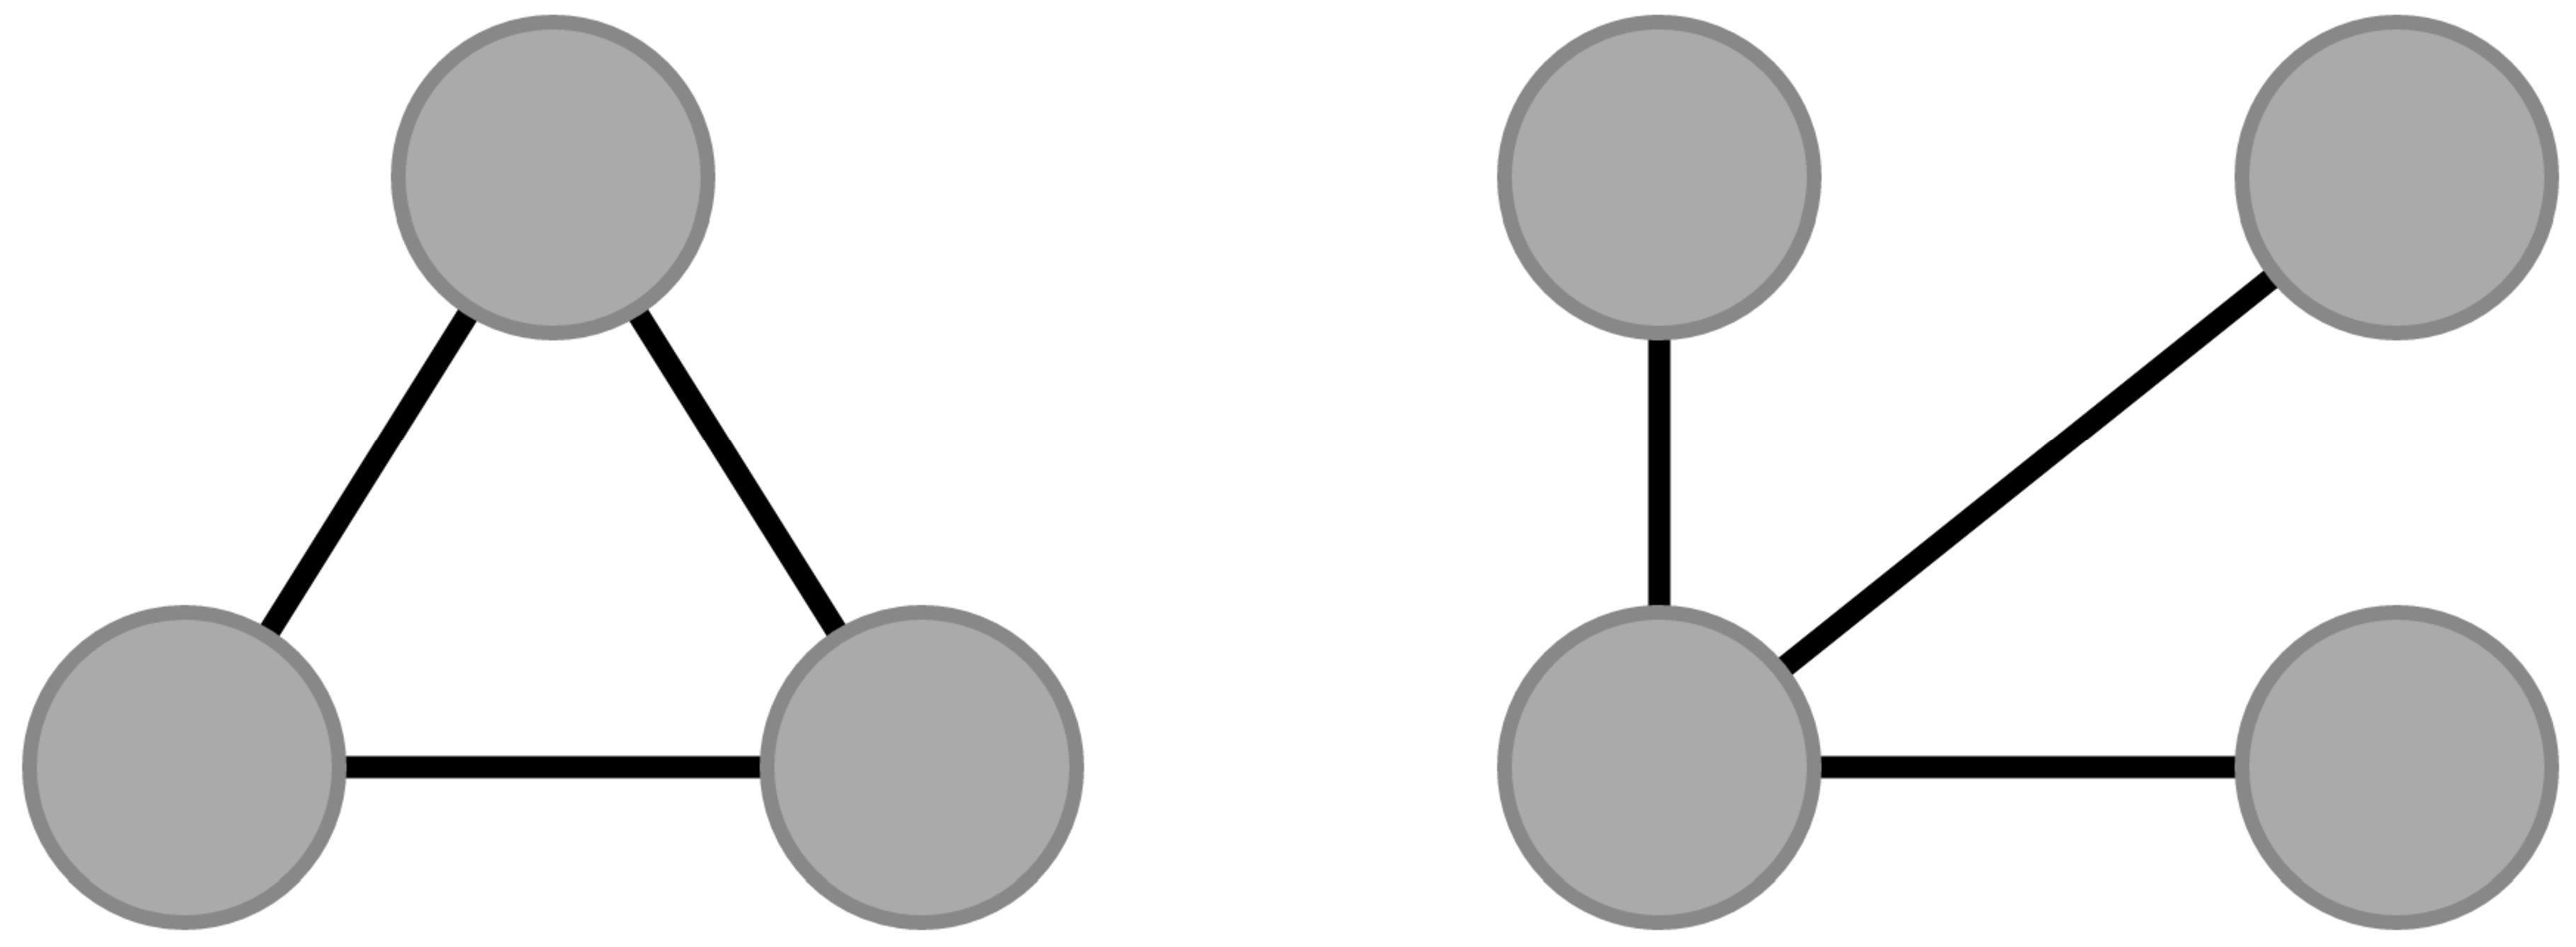
\includegraphics[width=6cm]{../figures/bad-criterion.pdf}
	\caption{Graphs $K_{3}$ and $K_{4}^{-3}$, respectively}\label{fig:bad-criterion}
\end{figure}

We can see that $G_2$ has both of these as minors. The transformation needed to see the minors is shown in figure \ref{fig:criterion-minor}. By contracting the dotted edges, vertices 1 and 4 would combine as well as vertices 3 and 5. We would have both $K_{3}$ and $K_{4}^{-3}$. Thus, this graph cannot be conflict-free colored with one color.

\begin{figure}[h]
	\centering
	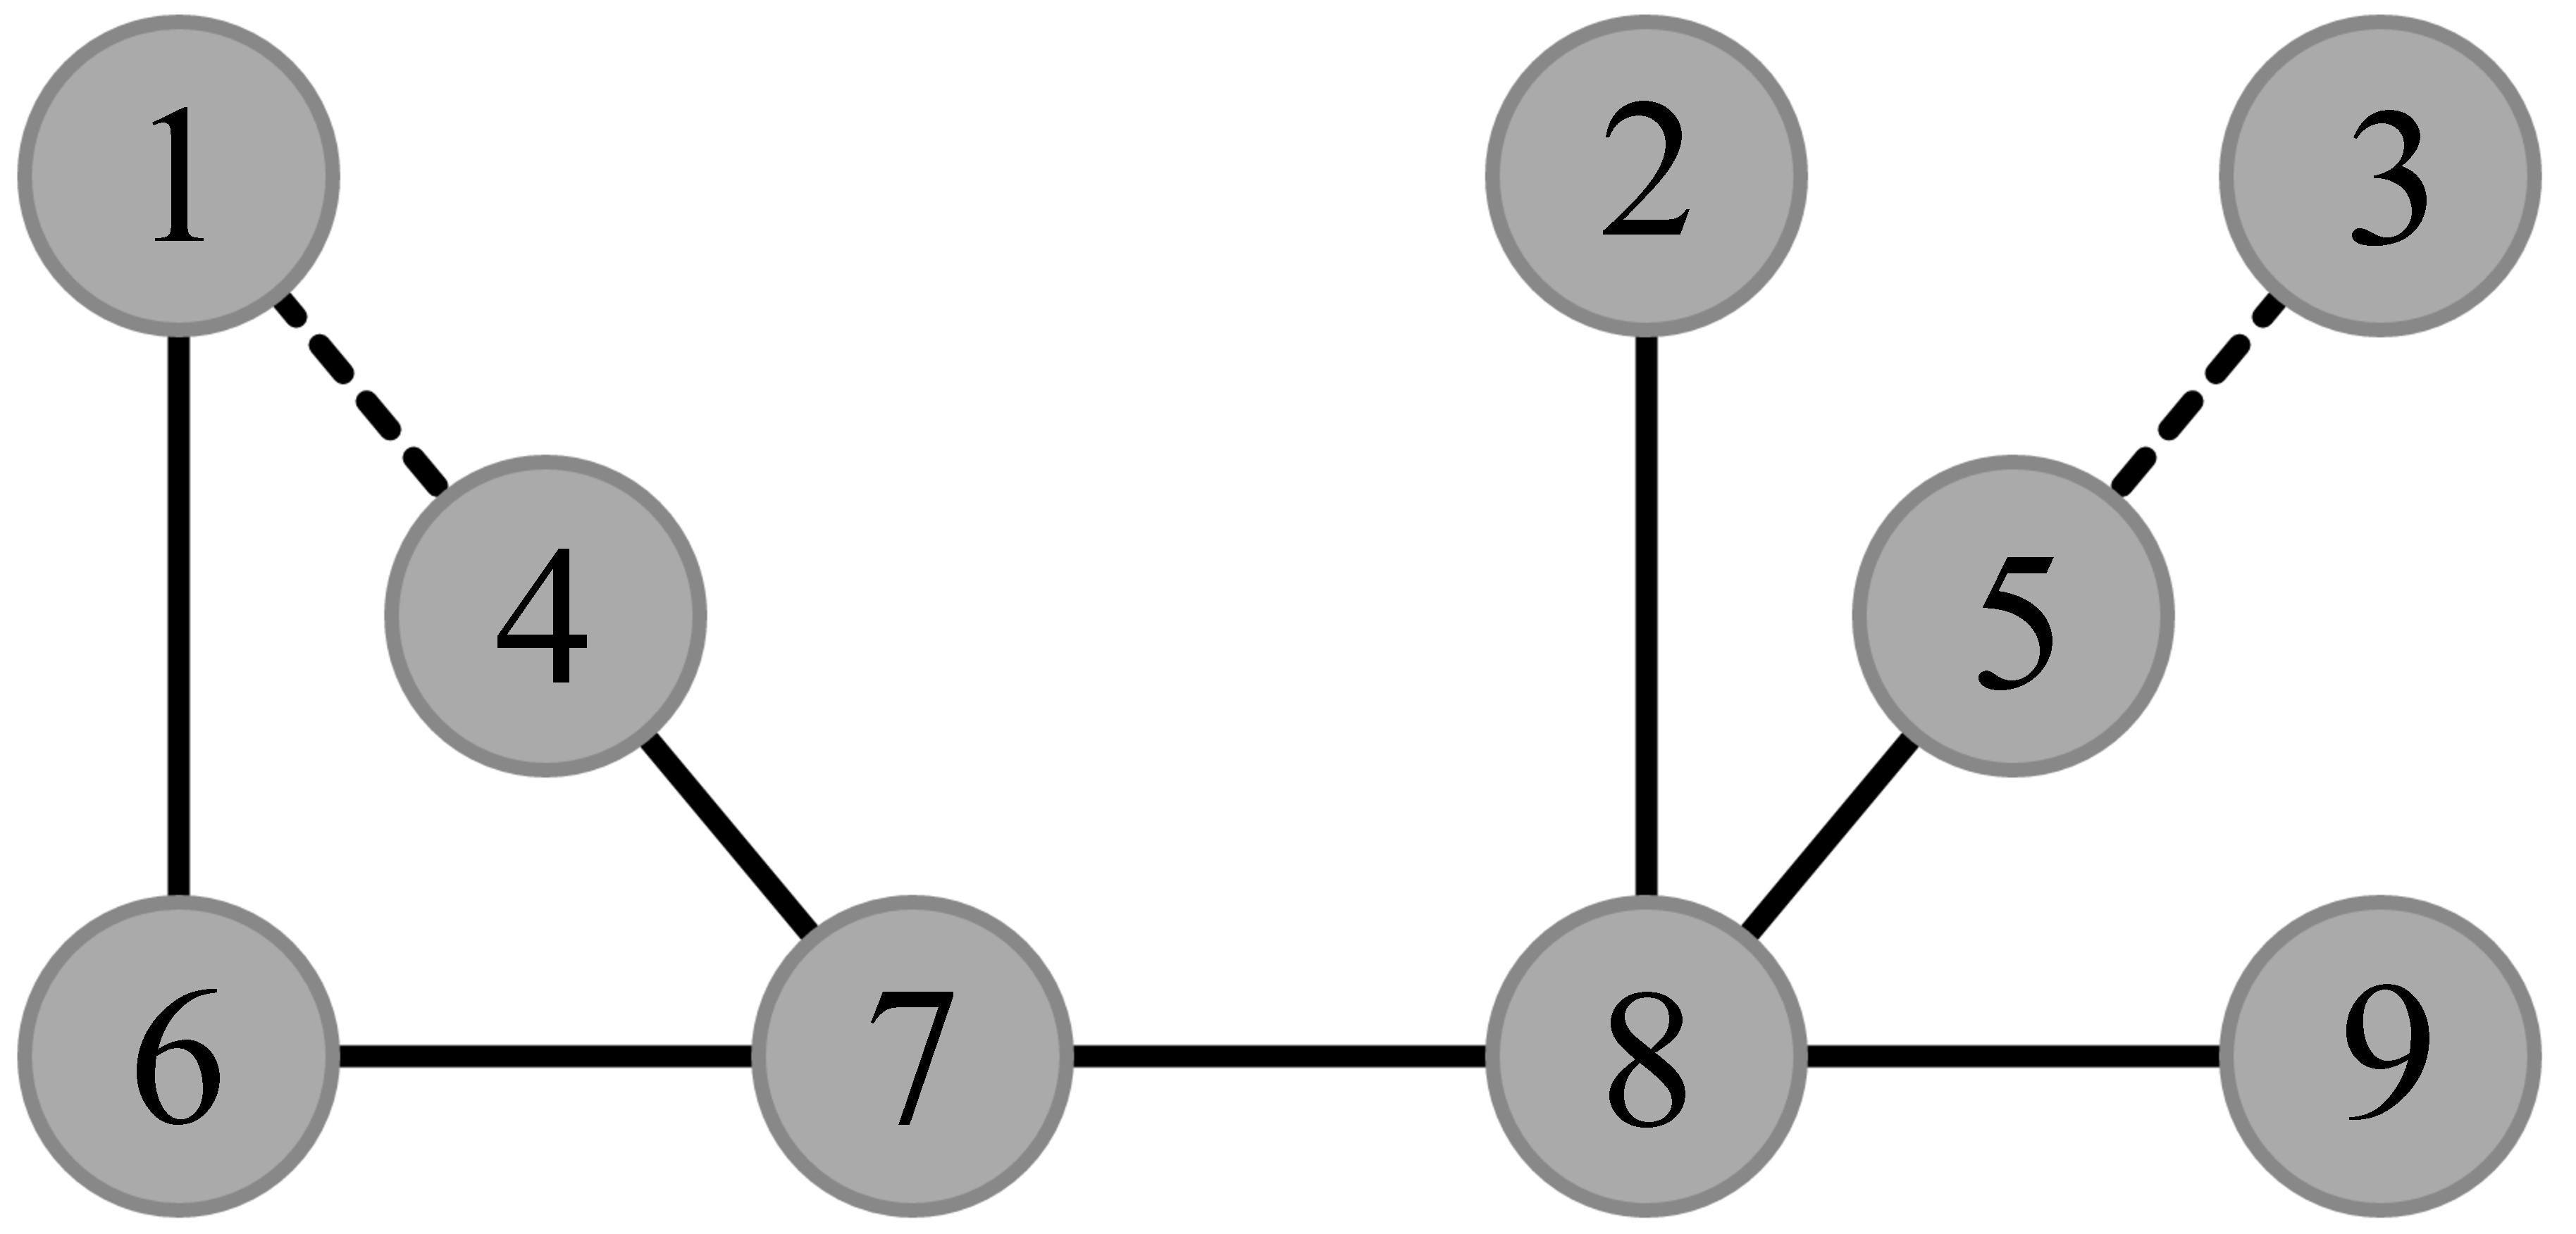
\includegraphics[width=6cm]{../figures/criterion-minor.pdf}
	\caption{How to transform $G_2$ to see the minors}\label{fig:criterion-minor}
\end{figure}

\subsection{Iterated Elimination of Distance-3-Sets}

\begin{algorithm}
\caption{Iterated elimination of distance-3-sets} \label{alg:elimination}
\begin{algorithmic}[1]
\State $i \gets 1$, $\chi \gets \emptyset$
\State Remove all isolated paths from $G$
\While{$G$ is not empty}
	\State $D \gets \emptyset$
	\ForAll{components of $G$}
		\State Pick a vertex $v$ and add it to $D$
		\While{$\exists u$ at distance $\geq 3$ $\forall v \in D$}
			\State Pick $u$ at distance 3 from some vertex in $D$
			\State $D \gets D \cup \{ w \}$
		\EndWhile
		\ForAll{$u \in D$}
			\State Color $u$ with color $i$
		\EndFor
		\State $i \gets i + 1$
		\State Remove $N[D]$ from $G$
		\State Remove all isolated paths from G
	\EndFor
\EndWhile
\State Color all removed isolated paths using color $i$
\end{algorithmic}
\end{algorithm}

\section{CF Coloring of Planar Graphs}


\section{Complexity of Coloring CF Graphs}



\section{Conclusion}
\label{sec:conclusion}

\section{Acknowledgments}
Thanks to Peter Dolan and Elena Machkasova for their feedback on this paper.

\bibliographystyle{abbrv}
\bibliography{../references}


\end{document}
